\section{Deployment Considerations}
\label{sec:analysis_deployment}

A service can be designed from the ground up with security in mind, implementing the strongest encryption \& access control mechanisms possible, but if deployed incorrectly the functioning security of the service can be completely undermined.
\vskip 0.5em
The University of Glasgow already provides Microsoft's SharePoint \citep{UofG2019} \& OneDrive \citep{UofG2019a} services as resource-sharing solutions to staff and students, however neither service offers truly granular access control \citep{Microsoft2019} and nor does either service offer a per-department service that the \acrshort{dcs} can implement for only its users.

This lack of granular access means that a user can not share a resource to all users enrolled in the same course, without manually inviting each user individually. By comparison, the \theResServer system would simply require creating a policy that grants access to users that have the attribute associated to that course, such as \texttt{`enrolled\_course \= 2003'}.

\subsection{Security of Public Resource Server}
\label{subsec:analysis_deployment_prs}

The \acrfull{prs} would need to be accessible to all 500+ users in the \acrshort{dcs} (\Cref{appendix:roles_users}) and able to process the uploading \& downloading of all encrypted resources. By design, the resource server would not be aware of the contents of any resources uploaded and would also be unable to execute any encryption or decryption tasks itself. The system would also reject uploads of any resources that are not yet encrypted.

Deployment of the \acrshort{prs} must be publicly accessible to all users in the \acrshort{dcs} and requires a limited level of security. The server does not necessarily require access to the \acrfull{mks} (see \Cref{subsec:analysis_deployment_mks} and \Cref{fig:deployment_diagram}) and can instead rely on manual updates completed via physical transfer by \acrshort{dcs} Admin staff.
\vskip 0.5em
Depending on the desired use, the resource server may be deployed for internal-use only and kept within the \acrshort{dcs} network or deployed with external access via the university's Campus network. Either scenario is considered safe as the resources on the server are implicitly secure due to the at-rest \acrshort{abe}.

Once deployed the system should integreate the university's Single Sign-On authentication system for basic access, which would help defend against attacks and other malicious attempts to disable or damage the system. Further consideration would need to be given to determining a suitable and effective method of completing backups of the encrypted resources but addressing that issue is outwith the scope of the project.

\subsection{Security of Master Key Server}
\label{subsec:analysis_deployment_mks}

Comparatively, the \acrfull{mks} represents the greatest risk to the \theResServer system, as the master \textbf{private} key stored within is capable of generating \& signing any private key. If the \acrshort{mks} becomes compromised, so does the entire system, since the master private key can be maliciously used to generate any arbitrary decryption key.

To combat this risk, the \acrshort{mks} is designed to be kept `offline' after initial setup is complete and the whole system has been successfully provisioned. This drastically reduces attack vectors to the server.

\begin{figure}[htp]
    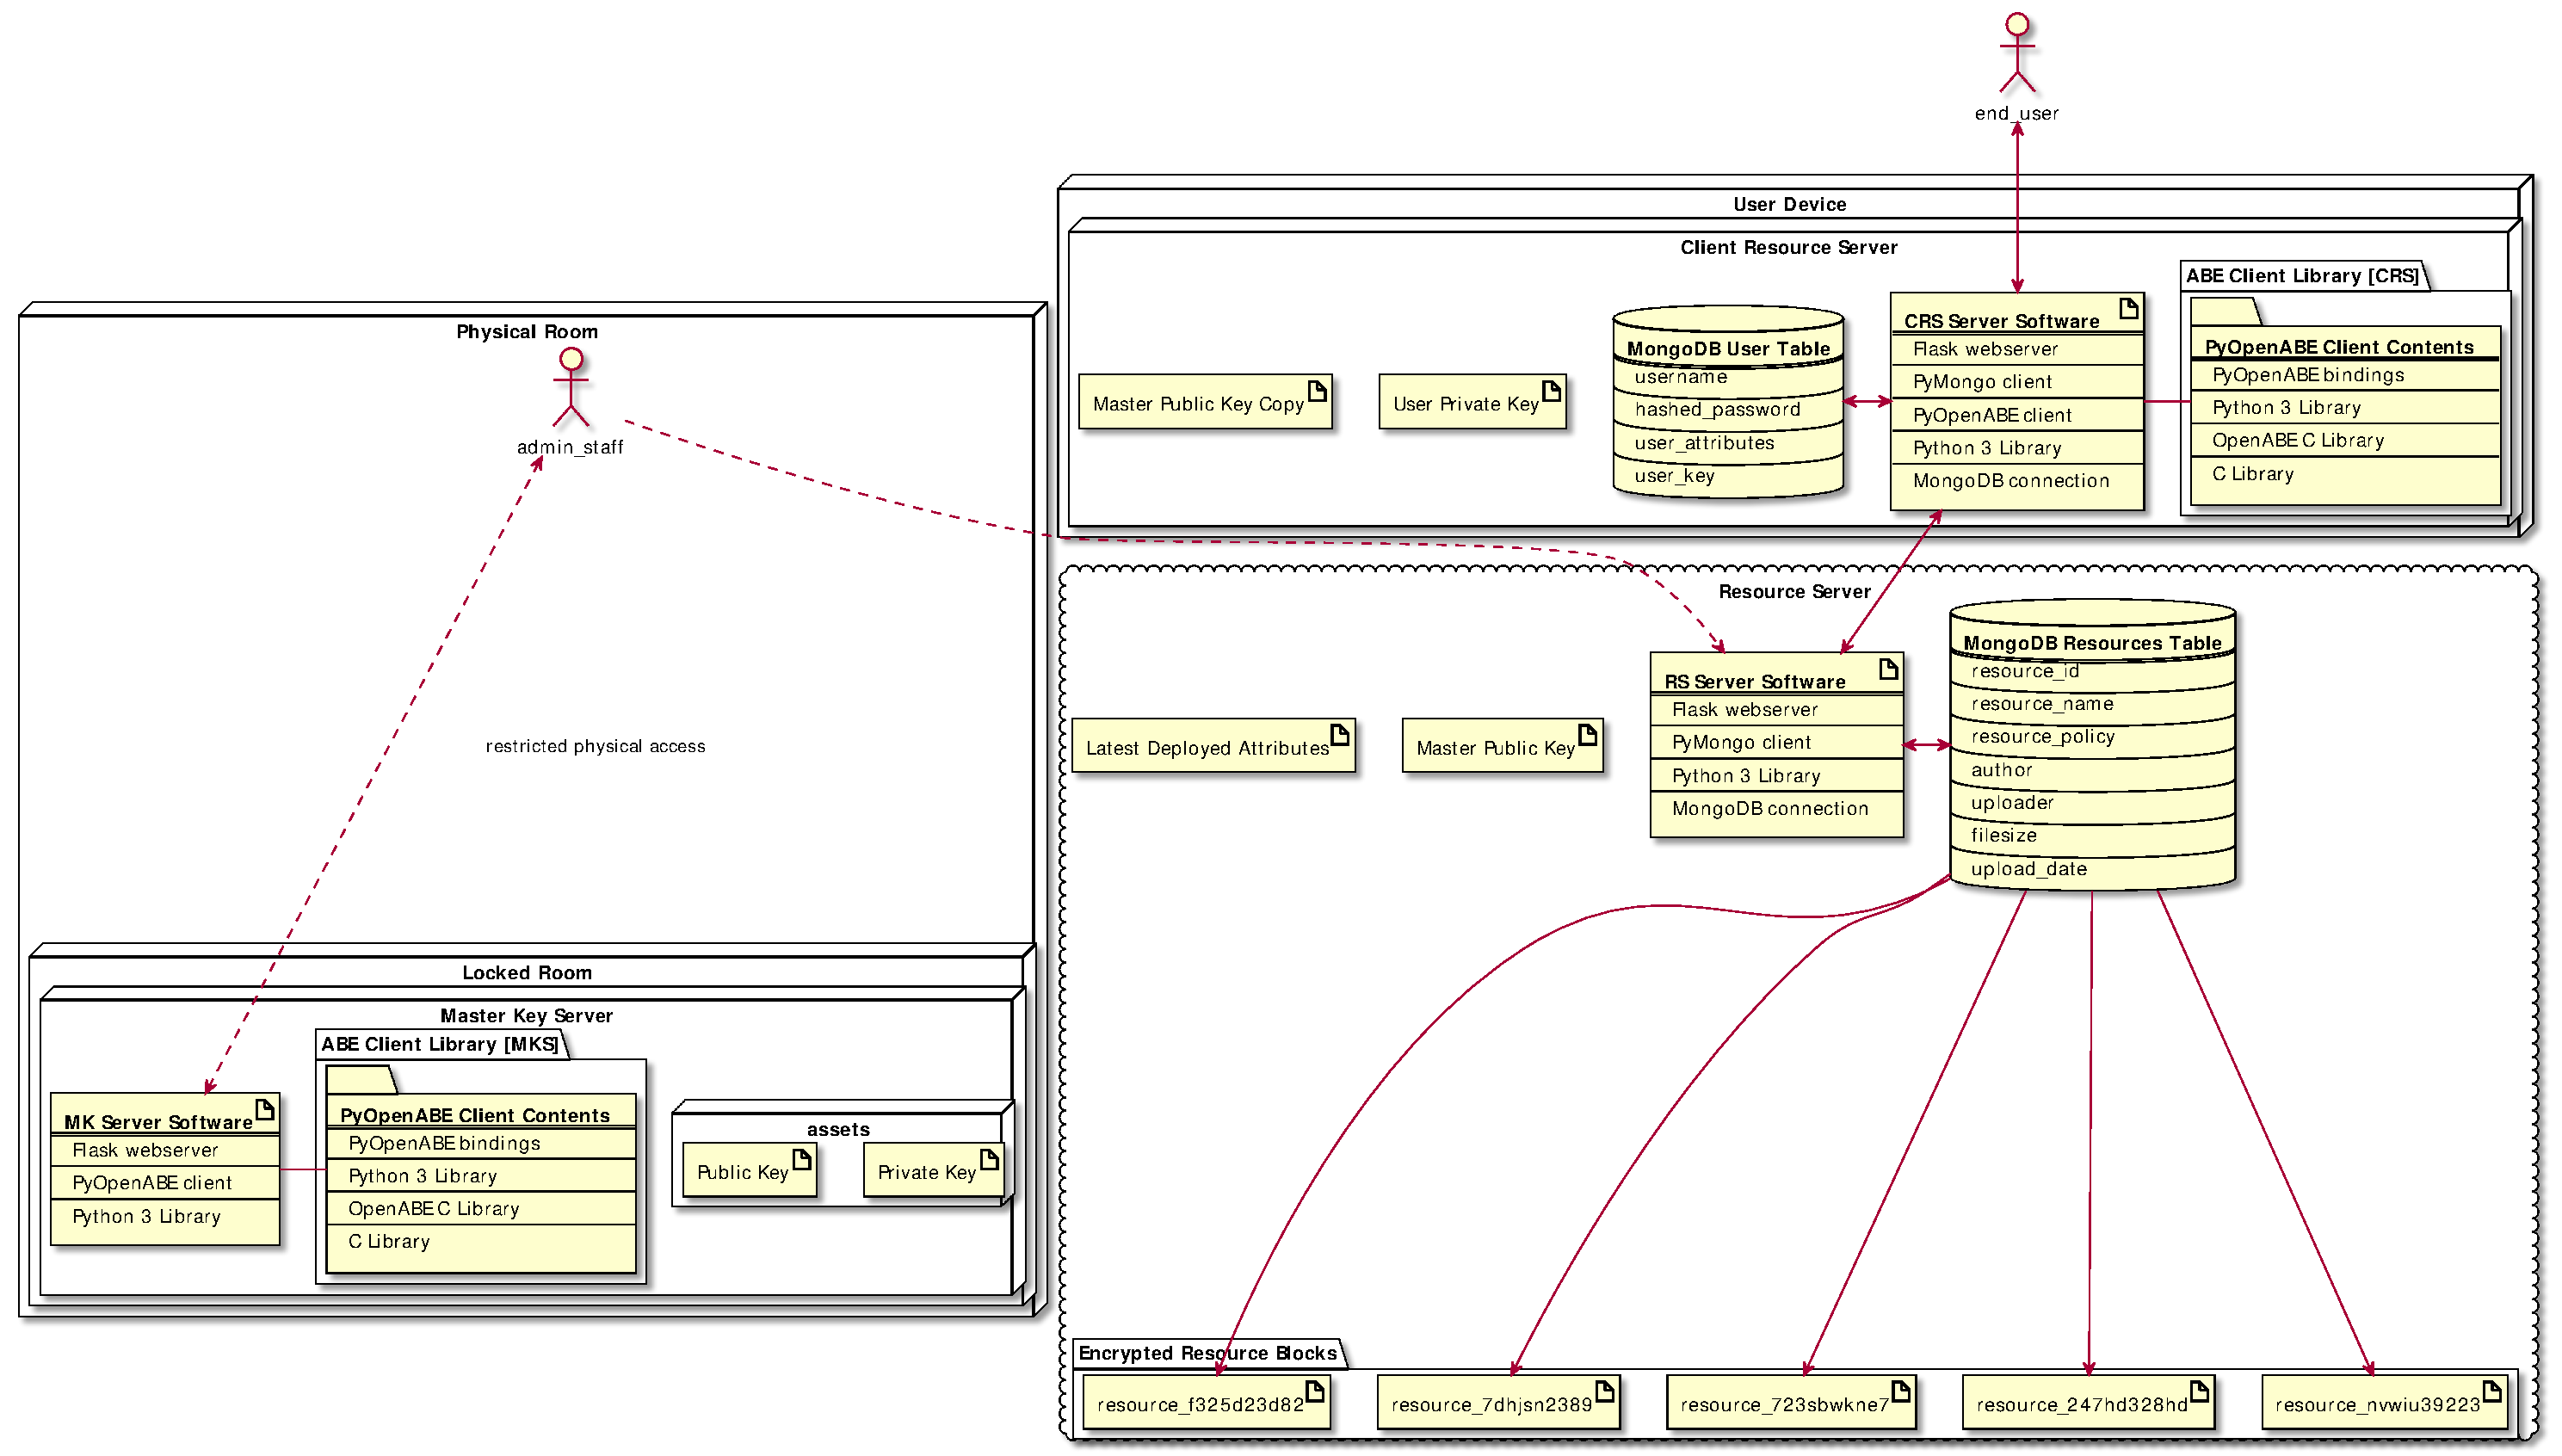
\includegraphics[width=\linewidth,keepaspectratio]{images/infrastructure/deployment.pdf}

    \caption{A deployment diagram of the \acrshort{dcs} \theResServer system. Both servers can be seen in context, with the \acrfull{mks} in its `offline' state and with physical access restricted to Admin staff. The \acrlong{prs} is shown receiving physical updates from the \acrshort{mks} (handled by Admin Staff) and communicating with a \acrlong{crs} running on a user's local device.}

    \label{fig:deployment_diagram}
\end{figure}

Physical access to the \acrshort{mks} remains a high risk concern. It was thus determined that physical access to the server must also be restricted, meaning the \acrshort{mks} would be deployed in a physically locked room with access only granted to \acrshort{dcs} Admin staff, as shown in \Cref{fig:deployment_diagram}.

The \acrshort{mks} would run on a UNIX \acrshort{os}, allowing for user authentication and system logging of events. Thus, in the event of a physical breach of security, a rogue party could not access the \acrshort{mks} to issue new keys. Additionally, if a rogue member of staff generates false keys, they would leave an auditable trail.

\subsection{Issuing User Keys}
\label{subsec:analysis_deployment_iuk}

From \Cref{subsec:analysis_deployment_mks}, the \acrfull{mks} generates \& signs decryption keys for the \theResServer system, using the stored master \textbf{private} key. Further, as discussed in \Cref{subsec:analysis_abe}, the decryption keys for the system are private user keys which contain embedded attributes that describe a user.

\begin{figure}[htp]
    \centering
    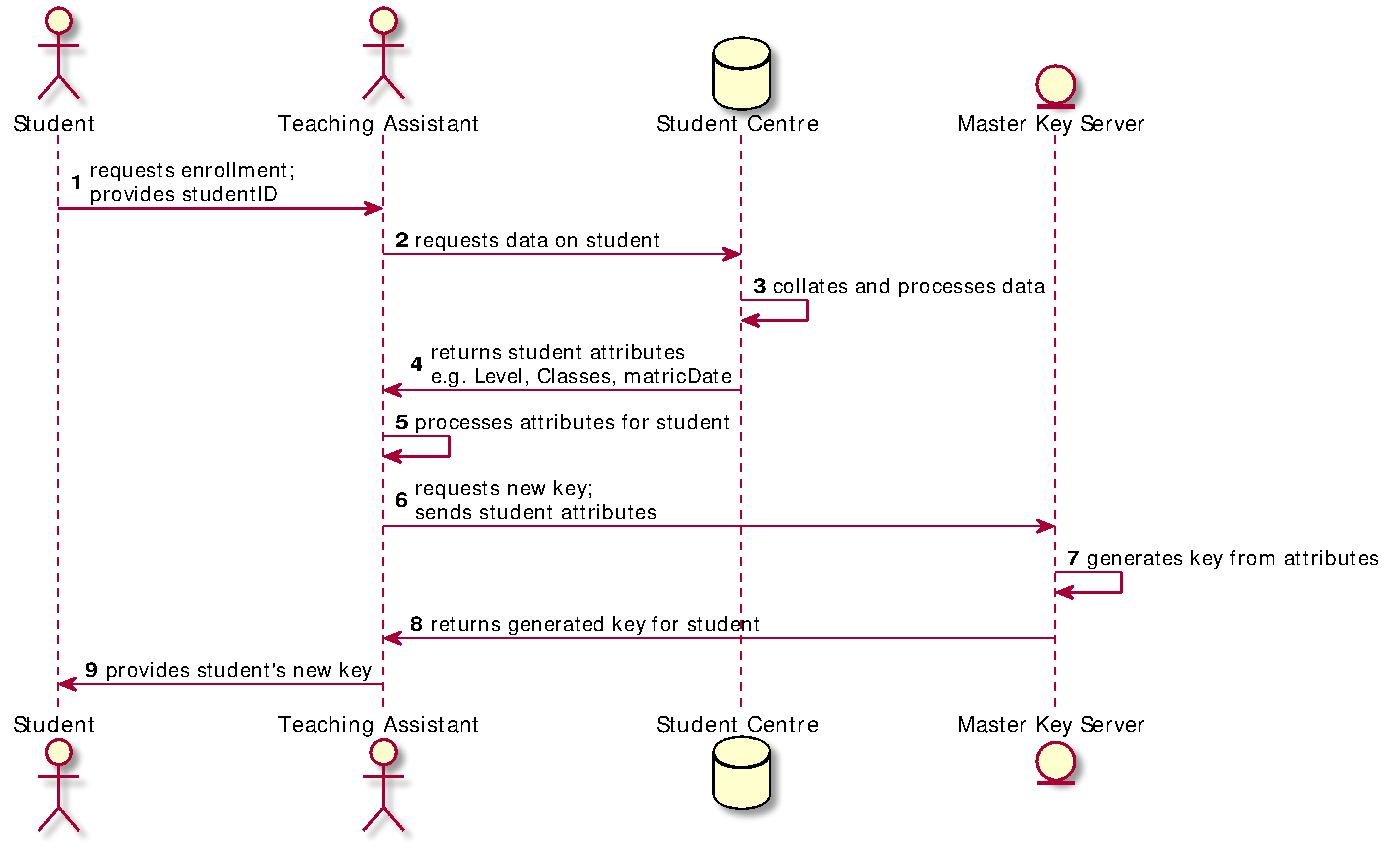
\includegraphics[width=\linewidth,keepaspectratio]{images/flow_of_info/enrollment_stu_sequence.pdf}

    \caption{A sequence diagram demonstrating the \theResServer enrolment process for a student.}

    \label{fig:enrolment_diagram}
\end{figure}

A user may enrol into the \theResServer system, by having a member of the \acrshort{dcs} Admin staff generate \& sign a new user key with their personal details from the \acrshort{mks}, see  and Appendix \ref{appendix:enrolment_diagram}.

\Cref{fig:enrolment_diagram} shows a student requesting a user key from the \acrshort{dcs} Teaching Assistant, whom verifies the student's identity and then retrieves their details from the Student Centre. The Teaching Assistant then processes the returned attributes for the \acrshort{mks}, and then requests a new key by providing the student's attributes. The \acrshort{mks} can be seen processing and then returning the newly generated key to the Teaching Assistant, whom finally provides the key to the student.
\vskip 0.5em
The \acrshort{mks} would be designed to \textit{validate} the attributes of a new user to ensure compatibility with encrypted resources and that all generated user keys are comparable. The \acrshort{mks} would not be designed to \textit{verify} the attributes of a new user.

It is instead assumed that the Admin staff are responsible for verifying both the identity of a user and that the attributes about to be assigned to them are correct; meaning both physical and login access to the \acrshort{mks} \textit{must only} be granted to trained members of staff.

The Admin staff member must physically transfer the newly created key from the \acrshort{mks} to the user via some form of hardware storage, such as a USB flash drive. Care would have to be taken to ensure that the \acrshort{mks} cannot become infected from malicious storage devices.
